\apendice{Documentación técnica de programación}

\section{Introducción}

En esta sección se hablará de aspectos más técnicos pensando en futuros desarrollos. Sirve como ayuda para entender el funcionamiento de la aplicación y de los pasos que se han llevado a cabo para conseguir estos resultados. Se detalla la estructura del programa, de la instalación y configuración de las herramientas necesarias y del proyecto y, por último, de las pruebas realizadas.

\section{Estructura de directorios}


\subsection{Aplicación}
Dentro se encuentra la carpeta \textbf{Thoth-Web}. En este directorio se almacenan los fichero del código fuente del proyecto en src, el directorio war, y también los test.

\begin{itemize}
	\item src
		\begin{itemize}
			\item client
			\item shared
			\item server
			\item módulo Login
			\item módulo GramaticaCS
		\end{itemize}
	\item test
		\begin{itemize}
			\item login
			
		\end{itemize}
	\item war
		\begin{itemize}
			\item imagenes
			\item login
			\item gramaticacs
			\item WEB-INF
		\end{itemize}
\end{itemize}	

Client esta organizado de la siguiente manera:

\begin{itemize}
	\item algorithms
	\item core
	\item gui
	\item login
	\item register
	\item main
	\item archivos de comunicación con el servidor
\end{itemize}	

Server contiene los siguientes elementos:
\begin{itemize}
	\item RegServlet.java
	\item GrammarServiceImp.java
	\item SessionServlet.java
\end{itemize}
\subsection{Prototipos}

En este directorio, se encuentran los prototipos hechos al inicio del proyecto. Sirven para entender el funcionamiento de diferentes aspectos de GWT como, creación de un proyecto, comunicación cliente-servidor y dos pruebas con el núcleo de Thoth cliente-servidor.

\begin{itemize}
	\item CorePrueba
	\item GWTProjectThree
	\item PrototipoCoreC-S
	\item StockWatcher
\end{itemize}	

\subsection{Documentación}

En este directorio se incluyen los la memoria y los anexos hechos con \LaTeX{}, así como las imágenes para documentarlos.

\section{Manual del programador}

\subsection{Instalación y configuración de GWT:}


Para poder trabajar con GWT \footnote{\url{http://www.oracle.com/technetwork/java/javase/downloads/index.html}}, se debe descargar el SDK de GWT proporcionado en la página web oficial. Los requisitos previos para crear un aplicación web con \emph{Google Web Toolkit} son básicamente dos: tener instalada la SDK de Java en su versión 1.6, o cualquiera superior a esta, y tener instalado también Apache Ant o en su defecto Apache Maven.

En mi caso, como trabajo con la plataforma Eclipse (versión 4.4.) al descargar el plugin de Google para Eclipse, este viene con GWT y la \emph{App Engine SDK}, todo junto. Se puede descargar desde la siguiente dirección \footnote{\url{http://www.gwtproject.org/usingeclipse.html}}.

Para instalar el plugin desde eclipse, solo tenemos que ir a <<\emph{help}>> y en el desplegable elegir la opción <<Install new software>>. Aparecerá una ventana con un recuadro en el que pone <<work with>> y nos da la opción de escribir una dirección web. Para consultar las direcciones según la versión de Eclipse sólo tiene que visitar \url{https://developers.google.com/eclipse/docs/download}.
Aparecerá los elementos que se pueden instalar, y ahí elegimos el \emph{plugin} de Google. Debemos esperar a que se instale y ya solo hará falta reiniciar Eclipse.

Como último paso, se debe referenciar la SDK de GWT y completar la instalación. Para habrá que ir a la opción <<window>> de la pantalla principal, hacer \emph{click} en preferencias y aparecerá una ventana con varias opciones. Buscamos la opción de Google y en \emph{web toolkit} y ahí añadir la referencia a la SDK con la dirección en la que se encuentra el archivo. Lo mismo hay que hacer para el \emph{App Engine} pero en este caso añadiendo la referencias al \emph{App Engine}.

El modo de trabajar con GWT es muy simple. Desde el \emph{plugin} podemos crear un nuevo proyecto dese <<New Web Application Project>>, darle un nombre y marcando las opciones del SDK y el App Engine.

 
\subsection{Parser JavaCC}

GWT esta compuesto por una parte cliente, que es la que será traducida a JavaScript, y otra servidor escrita en Java y que no se traducirá. En un principio se prueba a incluir toda la aplicación dentro del lado del cliente, traduciendo todo a JavaScript. Pero como ya se ha dicho en otros apartados, GWT sólo soporta unas determinadas librerías en dicho lado y tiene algunas restricciones más\footnote{\url{http://www.gwtproject.org/doc/latest/DevGuideCodingBasicsCompatibility.html}.} que obligan a incluir el parser de JavaCC en el servidor, en vez del cliente.

Originalmente en el núcleo de Thoth, dentro del directorio <<grammar>>, colgaba un sub-directorio llamado <<parserjavacc>> en el cual se encontraba el \emph{parser} para la gramática. Es la parte más importante a lo que a la gramática se refiere, ya que permite reconocer si una gramática está bien construida o no.


\subsection{Comunicación cliente-servidor}
Una vez alojado en el servidor el \emph{parser} habrá que establecer una comunicación entre la parte del ciente en la que habrá un método que llame a la funcionalidad que se desee del servidor.

Para hacerlo, GWT utiliza la técnica denominada por sus siglas en inglés RPC o llamada de procedimiento remoto (\emph{Remote Procedure Call}) que tiene una estructura similar a la siguiente ilustración \ref{fig:5.1}.

\begin{figure}[h]
\centering
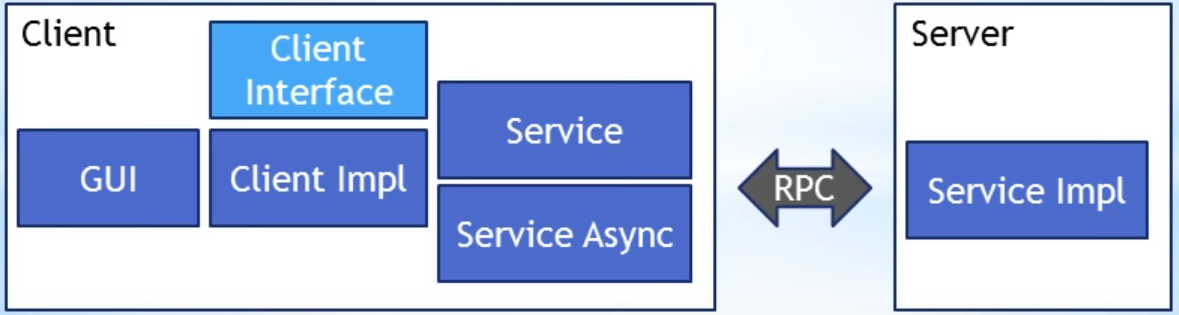
\includegraphics[width=0.65\textwidth]{RPC}
\caption{Arquitectura RPC simple.}
\label{fig:5.1}
\end{figure}

Del lado del cliente tenemos, en este caso, una interfaz gráfica de usuario (GUI), una clase dedicada a hacer las llamadas RPC (ClienImpl), dos interfaces que definen los métodos (\emph{Service} y \emph{ServiceAsync}), una clase con los métodos en el lado del servidor (serviceImpl) y por último una interfaz, que no es esencialmente necesaria (ClientInterface). 

En términos generales, para utilizar el \emph{parser} de la gramática, que es quizá la clave de todo, hay que llamar al servidor y establecer una comunicación. Es ahí donde utilizamos la clase <<GrmmarServiceClientImp>> que hace las llamadas a las interfaces necesarias hasta llegar al servidor. Esta clase es un nexo de unión entre la parte del núcleo, que ese encuentra en el servidor, y la parte del cliente, que contiene lo visual y las acciones de los botones entre otros. La comunicación queda representada en el diagrama \ref{fig:5.2}.

\begin{figure}[h]
\centering
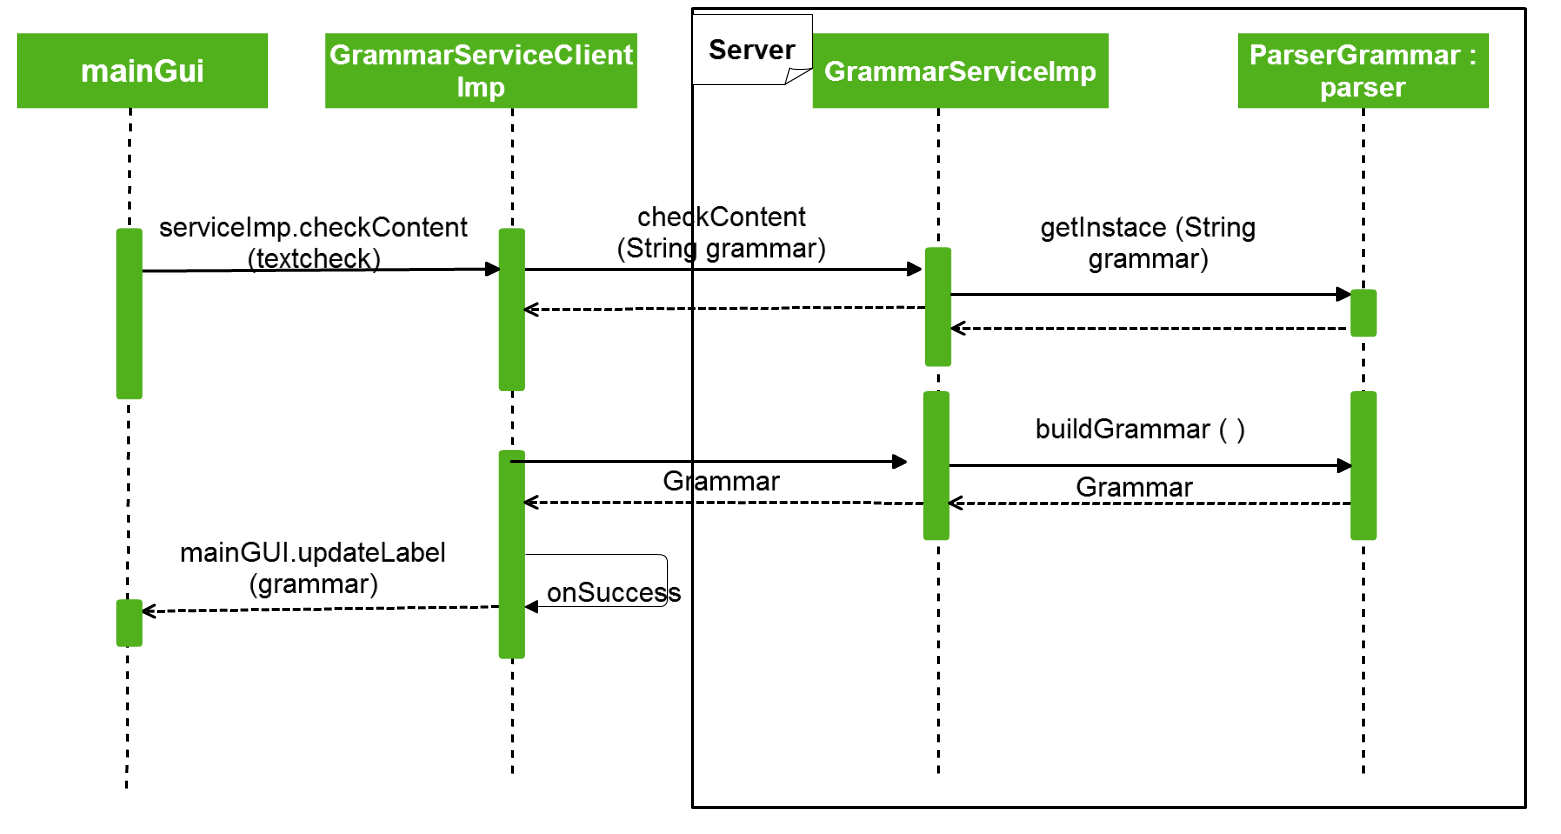
\includegraphics[width=1.1\textwidth]{ParserDiagram}
\caption{Diagrama sobre la comunicación entre el cliente y el servidor en GWT.}
\label{fig:5.2}
\end{figure}

Dentro de la clase <<GrammarServiceClientImp>> hay tres constructores según le pasemos una gramática, un texto, simplemente ningún parámetro. El atributo url es simplemente la localización del \emph{servlet} que se utiliza para la comunicación RPC. Estos detalles se aprecian mejor en el diagrama de clases que muestra la imagen \ref{fig:5.3}.

\begin{figure}
\centering
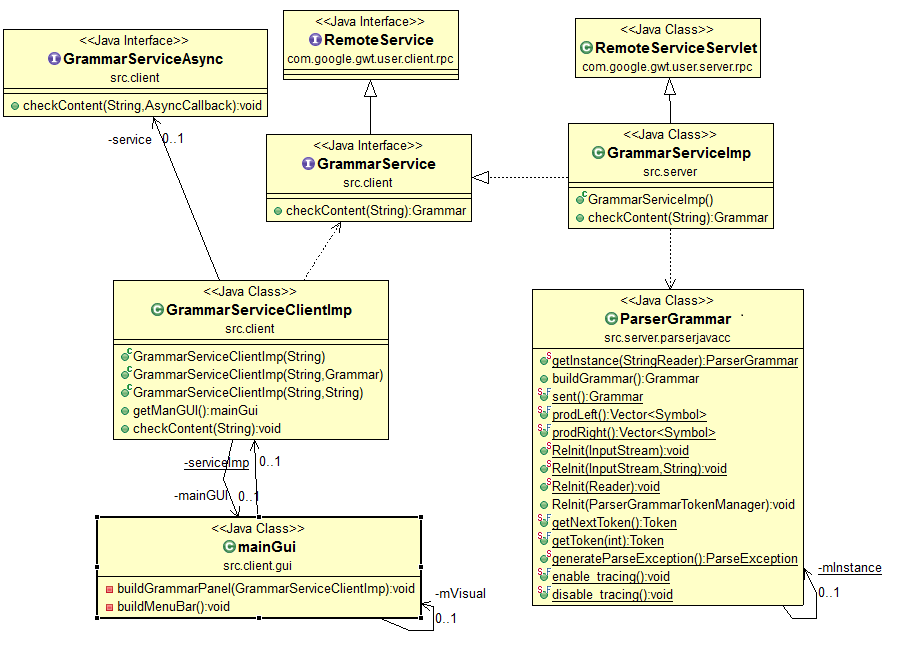
\includegraphics[scale=0.9]{Parser-ClassDiagram}
\caption{Diagrama de clases que muestra como utiliza el parser de la gramática. Diagrama realizado con ObjectAid.}
\label{fig:5.3}
\end{figure}

Una vez hechos todos estos pasos, es posible que no funciona nada, es más, dará un error del tipo \textit{\emph{did you forget to inherit a required module?}}. Todos los errores parecidos a este tienen que ver con el archivo <<web.xml>> que se encuentra en todos los proyectos GWT dentro de la carpeta <<war>> en <<WEB-INF>>. En ese archivo tenemos que definir los \emph{servlets}, dándolos un nombre y especificando la dirección, dentro del proyecto, donde se encuentran. Después deberemos indicar la dirección del patrón, es decir indicar a que módulo pertenecen y con que nombre. Ese nombre se lo especificamos anteriormente en la interfaz <<GrammarService>> con el componente <<@RemoteServiceRelativePath(``nombre'')>>.

\section{Compilación, instalación y ejecución del proyecto}

Antes de empezar a hablar sobre compilación debemos contar con un proyecto en GWT, preferiblemente en Eclipse, habiendo instalado el \emph{plugin} de Google, el SDK de \emph{App Engine} para Java y el SDK de GWT.

Hace unos años Google contaba con un \emph{plugin} para algunos navegadores (Chrome y Firefox, no confundir con el \emph{plugin} de Eclipse) con los que se podía ejecutar el proyecto. Pero Google paró el mantenimiento. Afortunadamente los desarrolladores de GWT crearon \emph{GWT Super-Dev Mode} que permite ejecutar cualquier proyecto realizado con esta herramienta.

En la definición del módulo, para poder realizar la ejecución con \emph{Super-Dev Mode} debemos incluir la sentencia \textit{add-linker name=``xsiframe''}. Si no lo incluimos podemos incurrir en algún tipo de error al ejecutarlo.
Las definiciones de los módulos se encuentran en la raíz de la carpeta principal y tienen una extensión <<.gwt.xml>>. Es habitual que no se llegue a hacer la compilación porque no se han definido los \emph{servlets} dentro del archivo <<web.xml>>.
  
\begin{figure}
\centering
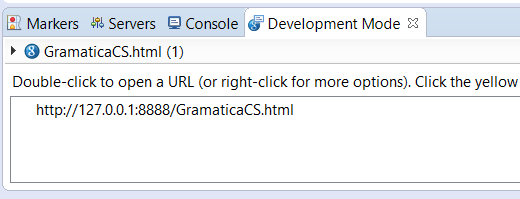
\includegraphics[scale=0.7]{SuperDevMode}
\caption{Dirección local que aparece al ejecutar en modo SuperDevMode.}
\label{fig:5.4}
\end{figure}

De esta forma una vez que se haya ejecutado en eclipse, se mostrará una dirección local que podemos abrir en nuestro navegador\ref{fig:5.4}. Este compilara los archivos HTML, y los JavaScript. Este proceso tardará unos segundo y cuando termine se mostrará la aplicación.

Si tenemos una base de datos, para poder acceder a ella, hay que coger la raíz de la dirección local, en nuestro caso <<http://127.0.0.1:8888/>>, y añadirle <<\_ ah/admin>>. Desde ahí podemos ver las entidades que hay, y en cada una de ellas los datos almacenados.

\subsection{Despliegue}

Por otro lado podemos desplegar la aplicación en \emph{App Engine}. Seleccionamos el proyecto que queramos, y nos vamos al \emph{plugin} de Google donde hacemos click en <<Deploy App Engine>> como muestra la imagen \ref{fig:5.5}. A continuación debemos dar un nombre al proyecto y en <<App Engine project settings...>> especificamos el identificador. Para hacerlo, debemos crear una cuenta aquí\footnote{\url{https://console.cloud.google.com/appengine}} y crear un proyecto. Automáticamente se le asignara un ID y ese es el que debemos introducir \ref{fig:5.6}. 
\begin{figure}
\centering
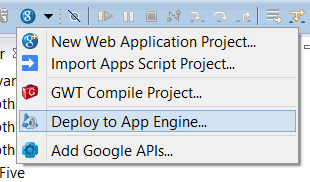
\includegraphics[scale=0.6]{Desplegar}
\caption{Acción de desplegar la aplicación con App Engine.}
\label{fig:5.5}
\end{figure}

\begin{figure}
\centering
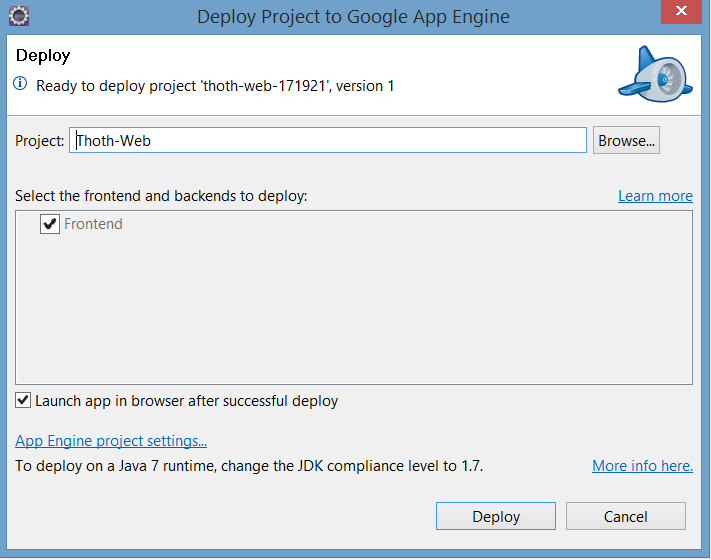
\includegraphics[scale=0.7]{Desplegar-dos}
\caption{Opciones de despliegue.}
\label{fig:5.6}
\end{figure}

Es importante que el SDK de Java sea el 1.7 ya que de lo contrario se producirá un error y no se desplegará la aplicación. La operación tardará un tiempo y ya solo quedará ir a la plataforma y ver si todo ha salido correctamente.

Si todo ha sido correcto, desde la nube podemos acceder a la base de datos como hacíamos en modo local, incluso con más detalle.

\section{Pruebas del sistema}


Las pruebas de sistema las hemos realizado con ayuda de Selenium \footnote{\url{http://www.seleniumhq.org/}}. Selenium es un entorno para realizar pruebas software en varios lenguajes, entre ellos, Java. Esta pensado para utilizarse en aplicaciones web. Para ello se puede descargar una extensión para el navegador, que digamos, grabará los pasos para cada test. Con esto se logra comprobar que el funcionamiento es correcto.

En este proyecto, hemos hecho pruebas sobre las sesiones, analizando, los siguientes casos:

\begin{itemize}
\item Inicio de sesión con \emph{email} y contraseña correctos. Se comprueba que el nombre del usuario aparece en el menú. Se cierra la sesión y se vuelve a la vista inicial.
\item Inicio de sesión con contraseña incorrecta. Se comprueba que no ha podido acceder. Se prueba si se muestra un mensaje de error.
\item Registro con correo no válido. Se comprueba que se muestra un mensaje de error. 
\item Registro válido. Se comprueba que se registra un usuario y el mensaje de que se devuelve.

\end{itemize}

También se han incluido test de prueba de gramáticas, pero en este caso son iguales a los que se realizaron en las anteriores versiones de Thoth \cite{thothv2}. 